\documentclass[10pt]{article}
\usepackage[margin=0.8in]{geometry}
\usepackage{times,graphicx,booktabs,amsmath,hyperref,url,microtype}
\title{Token-Level Uncertainty as a Predictor of Hallucinations in Large Language Models: A Paired Likelihood-Scoring Study}
\author{[Student Name]\\[Department / Institution]}
\date{}
\begin{document}
\maketitle
\begin{abstract}
Large language models can produce fluent but unsupported answers. Prior work suggests that token probabilities may provide useful uncertainty signals, but token surprisal is not equivalent to factual error: rare entities and alternative phrasings can also receive low probability. This paper presents a reproducible comparison of mean token negative log-likelihood (NLL) and maximum token NLL as ranking signals for benchmark-labelled hallucinated answers. We score paired reference and hallucinated answers from the question-answering configuration of HaluEval using \texttt{distilgpt2}, conditioning each answer on the same knowledge and question prompt. Source rows are split before candidate expansion, and the F1 threshold is selected on validation data only. We report AUROC, AUPRC, thresholded F1, precision, recall, and false-positive/false-negative analysis. \textbf{[REPLACE WITH A FACTUAL SUMMARY AFTER RUNNING THE EXPERIMENT; DO NOT INVENT METRICS.]}
\end{abstract}
\noindent\textbf{Keywords:} large language models, hallucination detection, token uncertainty, negative log-likelihood, HaluEval, evaluation

\section{Introduction}
Fluent language generation does not guarantee factual correctness. Hallucinated content may be unsupported by provided evidence or contradict reliable information. HaluEval was introduced as a benchmark for evaluating hallucination recognition in generated text \cite{li2023halueval}. A natural hypothesis is that a model's token probabilities contain signals that distinguish reliable from unreliable answers. However, token probability measures how well a sequence fits a model's conditional distribution, not whether its claims are objectively true.

The literature review motivating this study argues that uncertainty should be treated as a predictive feature rather than a direct truth score. Token-level methods can be affected by lexical rarity, tokenization, context, and calibration. Semantic entropy attempts to account for meaning-equivalent generations \cite{kuhn2023semantic,farquhar2024semantic}, while token-level uncertainty quantification has been studied directly for fact-checking \cite{fadeeva2024factchecking}. This project narrows that broad agenda to an executable comparison of two sequence-level aggregations.

\section{Research Question and Hypotheses}
\textbf{Research question:} On the HaluEval QA paired-answer benchmark, do mean token NLL and maximum token NLL distinguish benchmark-labelled hallucinated answers from reference answers when scored by the same causal language model?

\textbf{H1:} Higher mean token NLL will tend to rank hallucinated answers above reference answers. \textbf{H2:} Maximum token NLL will provide a different or complementary ranking signal to mean token NLL because it emphasizes the most surprising token. These are hypotheses to test, not assumed findings. No novelty claim is made.

\section{Related Work}
HaluEval provides paired reference and hallucinated responses for several generation tasks, including question answering \cite{li2023halueval}. Fine-grained factuality work such as FActScore decomposes long-form responses into atomic claims and assesses factual precision \cite{min2023factscore}. RAGTruth adds annotated hallucinations in retrieval-augmented generation \cite{niu2024ragtruth}. These resources illustrate that hallucination labels depend on task and annotation granularity.

Semantic uncertainty methods group generations by meaning rather than treating every wording as a distinct answer \cite{kuhn2023semantic,farquhar2024semantic}. Token-level uncertainty work has explored token probabilities and claim-conditioned probability for fact-checking \cite{fadeeva2024factchecking}. More broadly, calibration research shows that predictive confidence can differ from empirical correctness \cite{guo2017calibration}. This study does not implement semantic entropy, claim-conditioned probability, or calibration; these remain relevant extensions.

\section{Method}
\subsection{Dataset and paired design}
We use the QA configuration of \texttt{pminervini/HaluEval} accessed through Hugging Face Datasets. Each source row contains knowledge, a question, a reference answer, and a hallucinated answer. For each row, we form two candidates with the same prompt: a reference candidate labelled $y=0$ and a benchmark-labelled hallucinated candidate labelled $y=1$. The dataset card, schema, license, revision, and access date must be checked and recorded before final submission.

\subsection{Scoring model and predictors}
We use \texttt{distilgpt2} as a lightweight causal language-model scorer. It is a scoring model and is not assumed to be the model that generated the benchmark answers. Given a prompt $x$ and answer tokens $y_1,\ldots,y_T$, token NLL is
\[
\ell_t=-\log p_\theta(y_t\mid x,y_{<t}).
\]
We compute two response-level predictors:
\[
U_{\mathrm{mean}}=\frac{1}{T}\sum_{t=1}^{T}\ell_t,\qquad U_{\mathrm{max}}=\max_{1\leq t\leq T}\ell_t.
\]
Prompt tokens are excluded from the aggregation. A larger score is treated as a stronger signal of a hallucinated answer. These scores are not interpreted as probabilities of factual error.

\subsection{Splitting and evaluation}
Source rows are shuffled with a fixed seed and divided into 60\% training, 20\% validation, and 20\% test groups before the two candidates are expanded. This prevents paired candidates from the same question appearing in different splits. No predictive model is trained in this baseline; the training partition is retained to document the split protocol. The validation set selects the threshold maximizing F1. That threshold is applied unchanged to the held-out test set.

We report AUROC and AUPRC to assess ranking, and F1, precision, and recall at the validation-selected threshold. The final metrics must be copied from the generated \texttt{metrics.json} file. The script also saves per-answer scores, score-distribution plots, a response-length plot, and test-set error classifications.

\subsection{Implementation and reproducibility}
The experiment script records the model identifier, device, sample count, seed, split counts, runtime, per-candidate scores, and evaluation outputs. A smoke test on 50 pairs should be run before the planned 500-pair experiment. The final report must record actual package versions, hardware, runtime, warnings, and deviations. Results are based on the selected sample and should not be assumed to generalize automatically.

\section{Results}
\textbf{Do not submit this section with placeholders. Replace every bracketed item using the actual \texttt{results/main/metrics.json} and CSV outputs.}
\begin{table}[h]
\centering
\caption{Held-out test results. All entries must come from the executed experiment.}
\begin{tabular}{lccccc}\toprule
Predictor & AUROC & AUPRC & F1 & Precision & Recall\\\midrule
Mean token NLL & [TODO] & [TODO] & [TODO] & [TODO] & [TODO]\\
Maximum token NLL & [TODO] & [TODO] & [TODO] & [TODO] & [TODO]\\\bottomrule
\end{tabular}
\end{table}

The test set contains [TODO] source pairs and [TODO] answer candidates. The validation-selected threshold was [TODO] for mean NLL and [TODO] for maximum NLL. H1 was [supported/not supported/inconclusive based on outputs]. H2 was [supported/not supported/inconclusive], based on metric differences and score distributions. Avoid claiming statistical significance unless an appropriate test and uncertainty interval have actually been computed.

\begin{figure}[h]
\centering
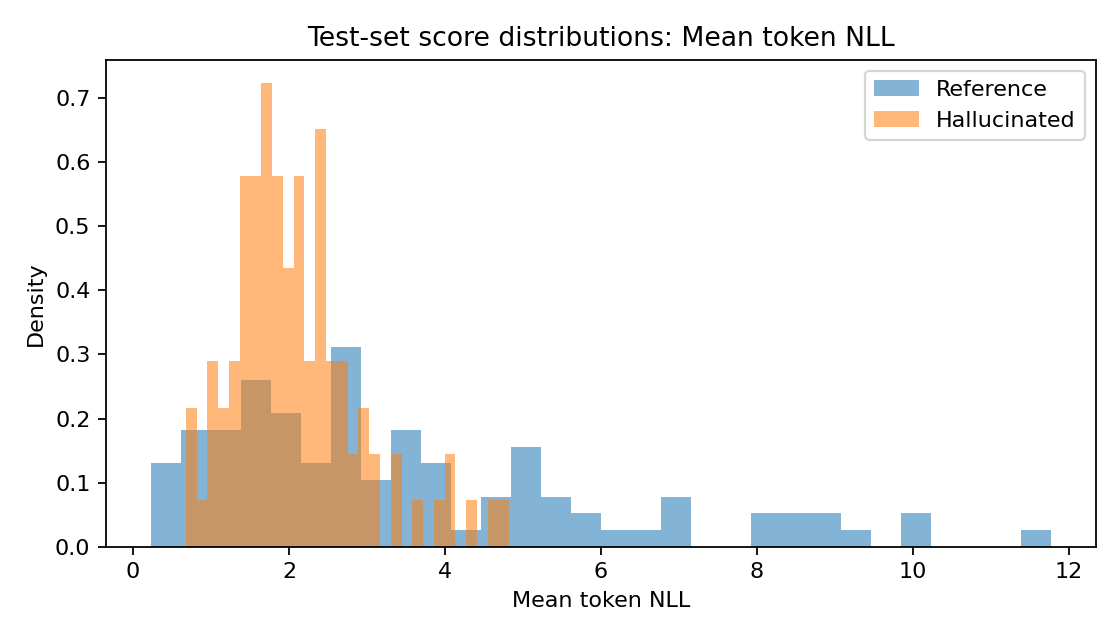
\includegraphics[width=.47\linewidth]{figures/mean_token_nll_distribution.png}
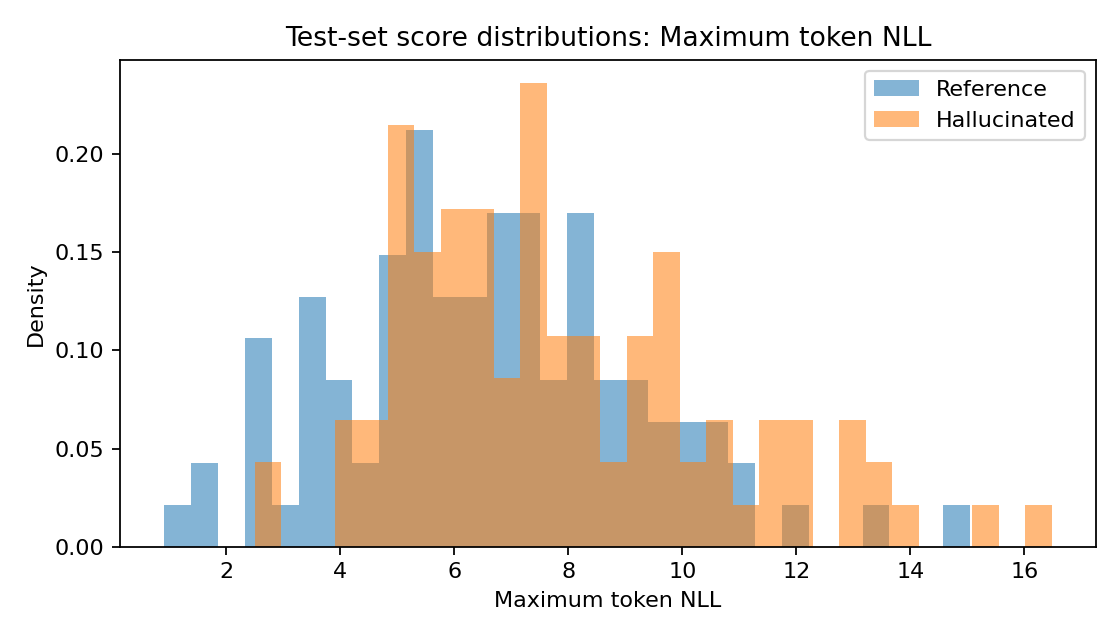
\includegraphics[width=.47\linewidth]{figures/max_token_nll_distribution.png}
\caption{Test-set score distributions. Copy actual generated PNGs from the results directory into this folder before compiling.}
\end{figure}

\section{Error and Sensitivity Analysis}
The script saves test predictions and classifies errors for mean NLL using the validation-selected threshold. Inspect \texttt{test\_error\_analysis.csv}. Report at least two false positives and two false negatives as qualitative examples, with answer text shortened if necessary and no unsupported claims about why the model failed. False positives are reference answers scored as suspicious; false negatives are benchmark-labelled hallucinations not flagged by the threshold.

The generated length plot supports a basic sensitivity check: compare response length with mean NLL and describe whether the relationship appears substantial. Also compare paired differences (hallucinated minus reference score) from \texttt{metrics.json}. These are descriptive analyses; do not infer causation from correlation. If truncation or prompt-length issues occur, document them and rerun with a justified protocol rather than silently discarding cases.

\section{Discussion}
Interpret findings narrowly. If one predictor performs better, this indicates that it ranked the benchmark's paired labels more effectively under this scoring model and sample; it does not establish that it measures truth directly. A difference between mean and maximum NLL may reflect local lexical surprises, response length, or the scoring model's distribution as well as factual errors. If performance is weak or hypotheses are unsupported, report that outcome rather than changing the test protocol after observing results.

\section{Limitations and Threats to Validity}
First, the sample is limited to one benchmark configuration and one scoring model. Second, the scorer may not match the model used to create the answers, so likelihood scores may reflect cross-model style differences. Third, benchmark labels do not replace independent fact verification. Fourth, NLL is sensitive to tokenization, answer length, and rare entities. Fifth, this experiment does not test token localization, calibration, semantic entropy, multilingual transfer, causal intervention, or retrieval-augmented generation. Sixth, a single random seed and small sample do not establish robust generalization. These limitations constrain the claims.

\section{Conclusion}
This paper defines a reproducible baseline comparison of mean and maximum token NLL for distinguishing HaluEval QA reference and hallucinated answers. Complete the conclusion only after examining held-out metrics and error cases. The outcome may be positive, negative, or inconclusive. Future work could add claim-level annotations, entropy or semantic-entropy predictors, multiple scoring models, bootstrap confidence intervals, and cross-domain evaluation.

\bibliographystyle{plain}
\bibliography{references}
\end{document}
